\section{Introduction}\label{sec:introduction}

Let \(S\) be a finite set and \(M=(m_{st})_{s,t\in S}\) a Coxeter
matrix.  Thus \(m_{ss}=1\) and, for distinct \(s,t\), the symmetric
entry \(m_{st}\) belongs to
\(\{2,3,\ldots\}\cup\{\infty\}\).
The Artin group \(A=A(W,S)\) has generators \(\sigma_s\), with the
relation equating the two alternating words of length \(m_{st}\)
whenever \(m_{st}<\infty\).  The Coxeter group \(W\) is the quotient
obtained by imposing \(\sigma_s^2=1\).
A subset \(T\subseteq S\) is \emph{spherical} if its standard Coxeter
parabolic \(W_T\) is finite.

The standard Artin Salvetti complex \(X(W,S)\) has one cell of
dimension \(|T|\) for each spherical subset \(T\), including its
vertex for \(T=\varnothing\).  Its attaching maps come from the
oriented Coxeter-Salvetti construction.  These include the braid
relations in dimension two and the spherical cells in all higher
dimensions.  We recall the full model in
Section~\ref{sec:topology}.

\begin{theorem}\label{thm:main}
For every Coxeter matrix on a finite set \(S\), the universal cover
of \(X(W,S)\) is contractible.  Equivalently,
\[
  \pi_n\bigl(X(W,S)\bigr)=0\qquad(n\ge2).
\]
The conclusion allows arbitrary finite labels, infinite labels,
and connected or disconnected diagrams.
\end{theorem}

Thus Theorem~\ref{thm:main} resolves the \(K(\pi,1)\) conjecture
for Artin groups with finitely many standard generators.
The theorem concerns the full Salvetti complex: its
higher-dimensional cells are part of both the statement and the proof.
Although the generating set is finite, the Coxeter group need not be.

Theorem~\ref{thm:main} also supplies the asphericity input in several
established implications.  In Section~\ref{sec:consequences}, the
finite-dimensional classifying space gives torsion-freeness, and the
center theorem of Jankiewicz--Schreve~\cite[Theorem~3]{JankiewiczSchreve2022},
together with Deligne's spherical center theorem~\cite[Theorem~4.21]{Deligne1972},
gives \(Z(A)\cong\Zbb^k\), where \(k\) counts the connected
Coxeter-diagram components whose Coxeter groups are finite.  For the
positive Artin monoid, defined by the same generators and braid relations
in the category of monoids, Dobrinskaya's equivalence~\cite{Dobrinskaya2002},
as reproved by Ozornova~\cite[Section~5]{Ozornova2013}, gives the natural
equivalence of its classifying space with that of the group.  We also apply Boyd's
conditional stability theorem~\cite[Corollary~B]{Boyd2020} to its exact
family obtained by attaching a growing type-\(A\) path to a distinguished
vertex of an arbitrary fixed finite diagram, with no other new edges.
Its constant-coefficient range is recorded in
Corollary~\ref{cor:boyd-stability}.

\subsection{Context}

In spherical type, the geometric model is the complement of the
complexified reflection hyperplanes modulo the free action of the finite
Coxeter group.  Its fundamental group is the Artin group, and the
conjecture asks whether this orbit space is aspherical
\cite[Section~2]{Brieskorn1973}.  Modern accounts conventionally attribute
the origins of the conjecture to Arnol'd, Brieskorn, Pham and
Thom~\cite[Introduction]{Paolini2026}.
The Salvetti model connects the pairwise braid presentation with a
finite-dimensional cellular space governed by spherical parabolics.
Asphericity makes this explicit complex a classifying space, so its
cells and attaching maps encode group-topological invariants.

For ordinary braid groups, the configuration-space arguments of
Fadell--Neuwirth and Fox--Neuwirth give the basic example
\cite[Section~8]{FoxNeuwirth1962}.
Deligne proved the spherical case using finite real reflection
arrangements~\cite{Deligne1972}.  The positive-monoid structure in
finite type was developed by Brieskorn--Saito and
Deligne~\cite{BrieskornSaito1972,Deligne1972}.
Salvetti's cellular constructions give the relevant arrangement and
Coxeter models~\cite{Salvetti1987,Salvetti1994}; standard Artin
parabolics embed by van der Lek's
theorem~\cite{VanDerLek1983}.  Paolini gives a recent account of the
spherical theorem and its cell structure~\cite{Paolini2026}.

Charney--Davis developed the modified Deligne complex, built from
spherical parabolic cosets, and its equivalence to the asphericity
problem~\cite[Section~1.5 and Corollary~3.2.6]{CharneyDavis1995}.
They proved the FC case, in which every subset with all pairwise labels
finite is spherical, and the dimension-at-most-two case
\cite[Theorems~4.3.5--4.3.6 and Proposition~4.4.5]{CharneyDavis1995}.
Here dimension means the largest size of a spherical subset, which can
be much smaller than the rank $|S|$.
Paolini--Salvetti resolved all affine types using dual noncrossing
partitions and discrete Morse theory
\cite[Theorem~8.15]{PaoliniSalvetti2021}, building on the dual and
Garside constructions of McCammond--Sulway~\cite{McCammondSulway2017}.

Recent geometric methods cover further broad classes.
Huang--Przytycki proved the dimension-at-most-three case and additional
specified higher-dimensional classes
\cite[Theorems~1.1 and~12.20]{HuangPrzytycki2025}.
Hoda--Huang proved the conjecture when every irreducible spherical
parabolic is of type $A$, $B$, or $I_2$
\cite[Theorem~1.3]{HodaHuang2026}.
Huang's tree reduction~\cite[Theorem~1.1 and Corollary~9.2]{Huang2026}
requires both asphericity for tree diagrams and the condition that every
special four-cycle of alternating types in their Artin complexes has a
common neighboring vertex.  Our proof uses the classical spherical-coset reduction
and contracts that poset directly for every finite-rank matrix.

The algebraic tools have a different ancestry.  Zigzag algebras and
braid actions by evaluation cones were developed by
Huerfano--Khovanov, Khovanov--Seidel and Seidel--Thomas
\cite{HuerfanoKhovanov2001,KhovanovSeidel2002,SeidelThomas2001}.
Heng--Licata extend these constructions to fusion categories and
arbitrary Coxeter labels~\cite[Sections~4--5]{HengLicata2024}.
We use a framed version of that construction, with explicit choices of
fusion factors and edge objects.  The extreme-degree tests adapt the
positive-divisor method of Brav--Thomas for ADE configurations of
$2$-spherical objects~\cite[Section~3]{BravThomas2011}; here the tests
also apply to right simples and must recover original colors after
unfolding.  The proofs record these adaptations at their points of use.

Heng--Licata also relate their distinguished fusion-equivariant
stability component to Artin hyperplane complements and formulate its
contractibility as a route to the \(K(\pi,1)\) conjecture
\cite[Theorem~7.7 and Conjecture~7.12]{HengLicata2024}.  Here we contract
the spherical-coset poset directly.  The local requirements are a
two-point comparison of spherical cosets and an obstruction to an isolated
positive harmonic layer.  They combine categorical cohomology with
harmonic extension to control the links of a single well-ordered filtration.

\subsection{The proof and its local estimates}

Write \(\mathcal D\) for the poset of spherical right cosets
\(A_Tx\), ordered by inclusion with nested types.
The classical spherical theorem, the parabolic embedding theorem,
and Quillen's Theorem~A identify its order complex up to homotopy
with the full Salvetti universal cover
(Lemma~\ref{lem:salvetti-comparison}).
The task is therefore to contract \(|\mathcal D|\).
We add the vertices in a well-order.  A vertex's \emph{earlier link}
is the part of its link already present, and a \emph{source} has
empty earlier link.  If all earlier links are empty or contractible,
each component is contractible and has exactly one source
(Lemma~\ref{lem:filtration-principle}).  Thus controlling links and
distinguishing sources are the two topological tasks.

We adjoin a frame vertex and construct a finite graded zigzag
algebra.  An Artin element acts by invertible bimodule complexes.
Its action on the frame projectives has finitely many
\emph{layers}, indexed by the sum of cochain and internal
generator degrees.  Their nonnegative weighted multiplicities
give vectors \(m^d(x)\), with coordinates indexed by the original
colors \(S\) and the frame \(o\).  An original color means one
standard generator.  The frame coordinate is always one in layer
zero and zero in every other layer.
For distinct original colors $i,j\in S$, the diagram weights are
$b_{ij}=2\cos(\pi/m_{ij})$ for finite labels, $b_{ij}=2$ for
infinite labels, and $b_{io}=b_{oi}=1$ for frame edges.
For a spherical coset \(A_Tx\), the multiplicities outside \(T\) are
independent of the representative.  Their \emph{harmonic extension}
\(p=p^d(A_Tx)\) retains those exterior coordinates and solves
\[
 2p_i=\sum_{j\ne i}b_{ij}p_j\qquad(i\in T).
\]
Sphericity guarantees a unique nonnegative solution.
These vectors define the height: compare the highest nonnegative
layer first, and at each level resolve equality of vectors by a
type-order rule before comparing lower layers.

Passing to a larger spherical coset replaces more coordinates by
harmonic values; passing to a smaller coset exposes actual layer
multiplicities.  Positive-definite Cartan forms control strict
comparisons.  A different rule is needed when the harmonic vector at a
level \(q>0\) restricts on a connected component of its positive support
to a null vector for that component's Cartan matrix, and all higher
harmonic vectors vanish on the component and its boundary.  At those
components we reverse the type-order tie.  This rule permits the
upper-link contraction, but requires closed inequalities in certain
lower links.

Call data \emph{capped at \(q\)} on a set of colors if there are no
generators there above layer \(q\).  The lower-link problem leads to
two kinds of sublevel inside a fixed spherical coset \(A_Tx\) whose
boundary data are capped at \(q\).  For a proper subcoset
\(A_Jz\subsetneq A_Tx\), compare the exposed
counts \(m_i^q(z)\), \(i\in T\setminus J\), with the harmonic values
\(p_i^q(A_Tx)\), requiring these colors to be capped at \(q\).
Strict inequalities define the strict sublevel.  When \(T\) is contained
in a support component of this null kind, we also need the special
closed sublevel,
which permits equality.
Proposition~\ref{prop:residue-sublevels} proves that the strict
sublevel is empty or contractible, and that the special closed
sublevel is nonempty and contractible.  Its induction again uses
earlier links, so every component has a unique source.  The two
algebraic estimates supply source uniqueness and closed-sublevel
nonemptiness, respectively.

First, at a putative source \(A_Jz\), a lower bound valid at every
capped representative of that coset turns the excess above
\(p^q(A_Jz)\) into a convex combination of subrepresentation dimensions
(Proposition~\ref{prop:convex-subobjects}).
A three-step tensor filtration then compares two such sources.
The resulting two-point inequalities have a sum equal to the
negative of a positive-definite Cartan quadratic form, forcing
equality of their harmonic data.  Right-simple complexes supply
a parabolic detector that then identifies the actual cosets.
This proves uniqueness of the possible sources
(Proposition~\ref{prop:candidate-uniqueness}).

Second, emptiness of a special closed sublevel would mean that
every capped representative has all its interior counts strictly
above the prescribed null harmonic values.  The Hom calculation
in Section~\ref{sec:rigidity}, together with convexity, controls
a finite sequence of twists that simplifies successive lower
layers while retaining the cap.  It forces the boundary of the
null component to vanish in each layer reached by this process.
The fixed frame supplies a nonzero boundary coordinate in layer
zero, so the lowest nonzero boundary layer lies at or below zero.
Reaching that layer, below \(q>0\), gives a contradiction.  This is
the isolated harmonic-layer obstruction
(Proposition~\ref{prop:isolated-layer}).
The tensor and Hom arguments are proved independently of the
subsequent topological contraction.

With these residue sublevels available, the earlier upper and lower
links in the global filtration are empty or contractible.
The vertex-filtration principle makes each component contractible;
rank-one cosets connect all singleton cosets and hence the entire
poset.  This proves Theorem~\ref{thm:deligne-contractible}, and
the Salvetti comparison proves Theorem~\ref{thm:main}.

Figure~\ref{fig:dependencies} summarizes these dependencies.

\begin{figure}[tbp]
  \centering
  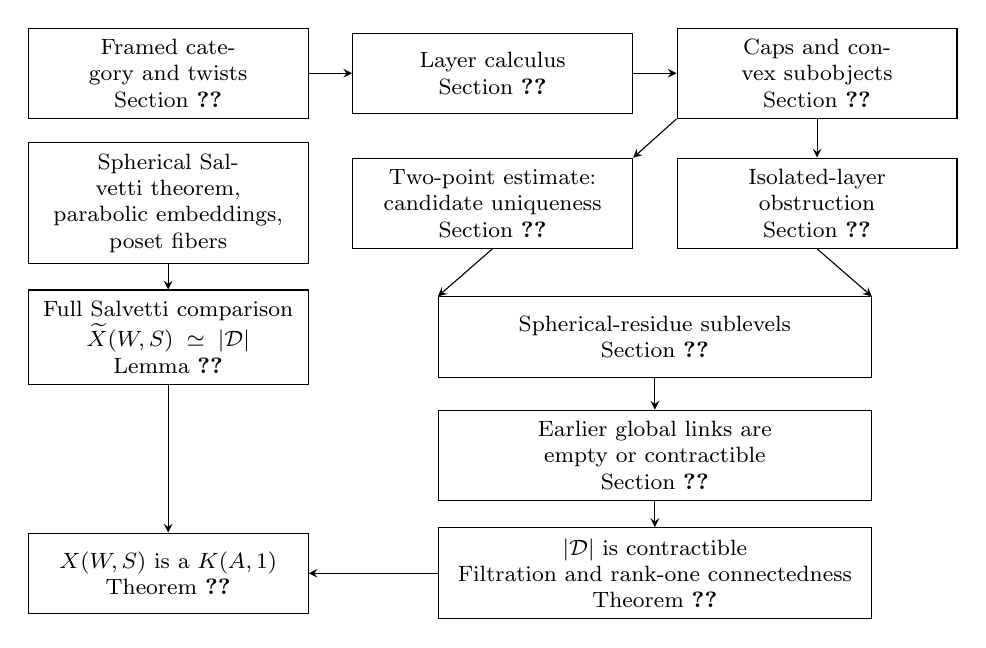
\begin{tikzpicture}[
      x=.01\linewidth,y=1cm,
      every node/.style={font=\footnotesize,align=center},
      result/.style={draw,thin,text width=.27\linewidth,
        minimum height=1.02cm,inner sep=4pt},
      wide/.style={result,text width=.43\linewidth},
      implication/.style={->,thin,>=stealth}
    ]
    \node[result] (category) at (0,0)
      {Framed category and twists\\Section~\ref{sec:category}};
    \node[result] (layers) at (34,0)
      {Layer calculus\\Section~\ref{sec:layers}};
    \node[result] (convexity) at (68,0)
      {Caps and convex subobjects\\Section~\ref{sec:height-data}};
    \node[result] (classical) at (0,-1.65)
      {Spherical Salvetti theorem,\\parabolic embeddings,\\poset fibers};
    \node[result] (two-point) at (34,-1.65)
      {Two-point estimate:\\candidate uniqueness\\Section~\ref{sec:two-point}};
    \node[result] (rigidity) at (68,-1.65)
      {Isolated-layer obstruction\\Section~\ref{sec:rigidity}};
    \node[result] (comparison) at (0,-3.35)
      {Full Salvetti comparison\\$\widetilde X(W,S)\simeq|\mathcal D|$\\
        Lemma~\ref{lem:salvetti-comparison}};
    \node[wide] (residues) at (51,-3.35)
      {Spherical-residue sublevels\\Section~\ref{sec:residues}};
    \node[wide] (links) at (51,-4.85)
      {Earlier global links are empty or contractible\\Section~\ref{sec:global}};
    \node[wide] (contractibility) at (51,-6.35)
      {$|\mathcal D|$ is contractible\\
        Filtration and rank-one connectedness\\
        Theorem~\ref{thm:deligne-contractible}};
    \node[result] (target) at (0,-6.35)
      {$X(W,S)$ is a $K(A,1)$\\Theorem~\ref{thm:main}};

    \draw[implication] (category) -- (layers);
    \draw[implication] (layers) -- (convexity);
    \draw[implication] (convexity.south west) -- (two-point.north east);
    \draw[implication] (convexity) -- (rigidity);
    \draw[implication] (two-point.south) -- (residues.north west);
    \draw[implication] (rigidity.south) -- (residues.north east);
    \draw[implication] (residues) -- (links);
    \draw[implication] (links) -- (contractibility);
    \draw[implication] (classical) -- (comparison);
    \draw[implication] (comparison) -- (target);
    \draw[implication] (contractibility) -- (target);
  \end{tikzpicture}
  \caption{The main dependencies.  The two algebraic estimates are proved
    before their use in the induction on spherical residues.  The classical
    comparison is independent of the height argument and transfers the
    resulting contraction to the full Salvetti universal cover.  Arrows
    display the main flow of the proof; the finite-type Coxeter and monoid
    inputs to the algebraic constructions are specified in the text.}
  \label{fig:dependencies}
\end{figure}


\subsection{Conventions and organization}

All posets are realized as their order complexes with the CW
topology.  All tensor categories and algebras are over \(\C\).
Complexes carry cochain and internal gradings; the total generator
degree is their sum.  Only cochain degrees determine differential
signs.  We use bimodule homotopy equivalences whenever a
nonprojective module will subsequently be tensored.
Subsets written with \(\subseteq\) need not be proper.

Section~\ref{sec:topology} fixes the topological model and the
classical inputs.
Sections~\ref{sec:category}--\ref{sec:height-data} construct the
algebra, its action, the layers and their convexity.
Sections~\ref{sec:two-point} and~\ref{sec:rigidity} prove the two
local estimates.
Sections~\ref{sec:residues} and~\ref{sec:global} establish the
sublevel theorem and the global contraction.
Section~\ref{sec:consequences} derives the structural consequences and
the homological-stability statement for fixed-core braid-tail families.
